\bgroup
\def\rone{28.8}
\def\rtwo{4.553}
\def\l{12.425}
Die Unit Telescopes des Very Large Telescope VLT der Europäischen
Südsternwarte (European Southern Observatory, ESO) auf
dem Cerro Paranal in Chile besteht aus einem Hauptspiegel $M_1$ mit
8.2\,m Durchmesser und Krümmungsradius $r_1=\rone\,\text{m}$, der das Licht
zum Sekundärspiegel $M_2$ wirft.
Dieser hat einen Durchmesser von 1.12\,m und einen Krümmungsradius
von $r_2=\rtwo\,\text{m}$.
Die Entfernung zwischen Hauptspiegel und Fangspiegel beträgt
$l=\l\,\text{m}$.

\begin{figure}[h]
\centering
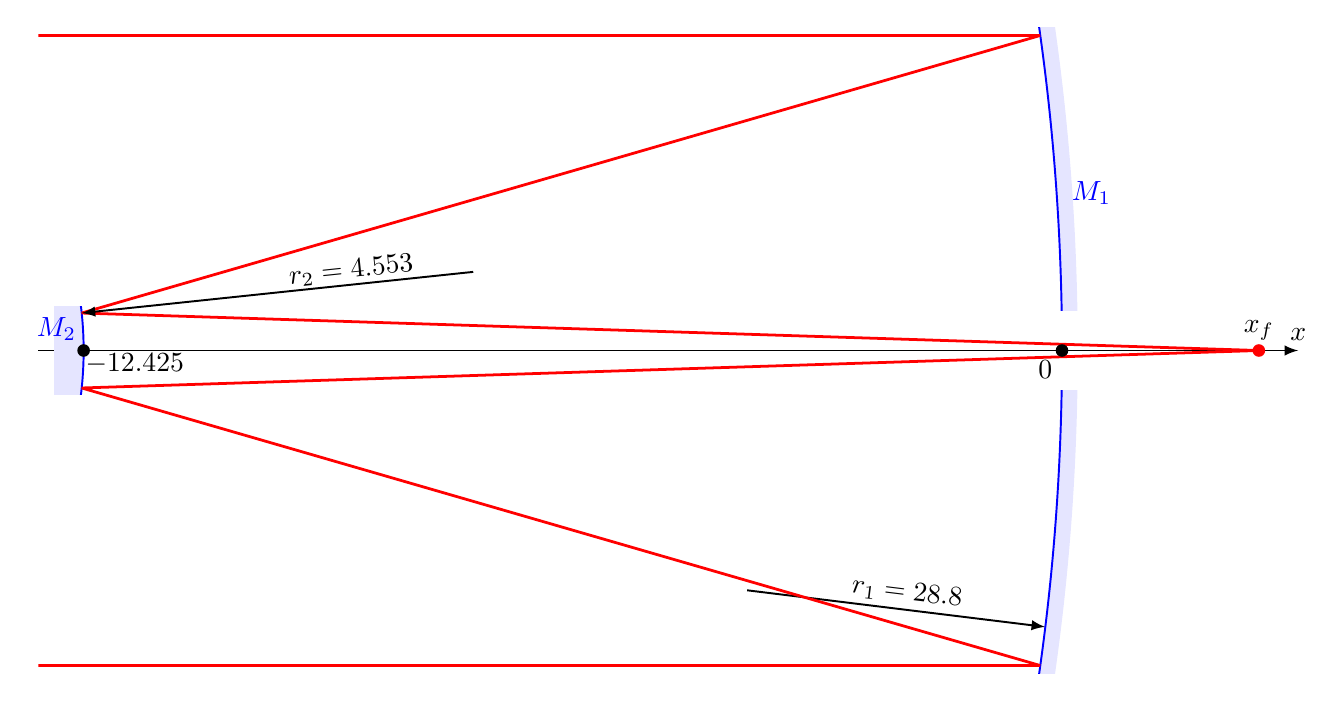
\begin{tikzpicture}[>=latex,scale=1.0]
\begin{scope}
\clip (-4,-4.1)--(1,-4.1)--(1,4.1)--(-4,4.1)--cycle;
\fill[color=blue!10] (-\rone,0) circle[radius={\rone+0.2}];
\fill[color=white] (-\rone,0) circle[radius=\rone];
\draw[->,line width=0.7pt] (-\rone,0) -- ({\rone*(cos(-7)-1)},{\rone*sin(-7)});
\draw[color=blue,line width=0.7pt] (-\rone,0) circle[radius=\rone];
\end{scope}
\fill[color=white] (-1,-0.5)--(1,-0.5)--(1,0.5)--(-1,0.5)--cycle;
\draw[->,line width=0.7pt] (-13,0)--(3,0) coordinate[label={$x$}];

\begin{scope}
\clip (-12.8,-0.56)--(-12,-0.56)--(-12,0.56)--(-12.8,0.56)--cycle;
\fill[color=blue!10] ({-\l-\rtwo},0) circle[radius={\rtwo}];
\draw[color=blue,line width=0.7pt] ({-\l-\rtwo},0) circle[radius={\rtwo}];
\end{scope}

\draw[color=red,line width=1pt,line join=bevel]
	(-13,4.0)
	--({sqrt(\rone*\rone-4.0*4.0)-\rone},4.0)
	--({-\l+\rtwo*(cos(6)-1)},{\rtwo*sin(6)})
	--(2.5,0);
\draw[color=red,line width=1pt,line join=bevel]
	(-13,-4.0)
	--({sqrt(\rone*\rone-4.0*4.0)-\rone},-4.0)
	--({-\l+\rtwo*(cos(6)-1)},{-\rtwo*sin(6)})
	--(2.5,0);
\fill[color=red] (2.5,0) circle[radius=0.08];

\node at ({-\l-0.1},0.08) [below right] {$-\l$};
\node at (0,0) [below left] {$0$};
\fill (-\l,0) circle[radius=0.08];
\fill (0,0) circle[radius=0.08];

\node at (-2.0,-3.34) [above,rotate=-7] {$r_1 = \rone$};

\draw[<-,line width=0.7pt]
	({-\l+\rtwo*(cos(6)-1)},{\rtwo*sin(6)})
	--
	({-\l-\rtwo+(\rtwo+5)*cos(6)},{(\rtwo+5)*sin(6)});
\node at (-9,0.75) [rotate=6,above] {$r_2=\rtwo$};
\node at (2.5,0) [above] {$x_f$};

\node[color=blue] at (-12.396,0) [above left] {$M_2$};
\node[color=blue] at (0, 2) [right] {$M_1$};

\end{tikzpicture}
\caption{Optische Parameter und Strahlengang eines VLT Unit Telescope
auf dem Cerro Paranal in Chile.
\label{10000058:fig}}
\end{figure}

Man kann die Matrixoptik (paraxiale Näherung) auch für Spiegel verwenden,
indem man als Brechungsindex $n=-1$ wählt.
\begin{teilaufgaben}
\item
Berechnen sie die $x$-Koordinate $x_f$, bei der von links einfallende
parallele Strahlen fokusiert werden.
Dies ist die Position der Brennebene im sogenannten {\em Cassegrain Fokus},
hier müssen die Messinstrumente montiert werden.
\item
Bei welcher $y$-Koordinate $y_0$ kreuzt ein Strahl,
der mit einem Winkel von $1''$
auf dem Hauptspiegel auftrifft, die in a) berechnete $x$-Koordinate $x_f$ der
Brennebene.
\item
Die effektive Brennweite ist die Entfernung $f$, bei der ein Winkel von
$1''$ zu einem Abbild der Grösse $y$ führt, also $y_0=f\sin 1''$.
Berechnen Sie die Brennweite eines VLT Unit Telescope im Cassegrain Fokus.
\end{teilaufgaben}

\themaS{Matrixoptik}

\begin{loesung}
Um die gestellten Fragen über das optische System des VLT Unit Telescope
zu beantworten, müssen die Transfermatrizen für die Spieglungen 
bestimmt werden.
Für die Spiegelungen sind dies die Matrizen
\[
B_1=B(1,-1,-r_1)=
\begin{pmatrix}
1&0\\-\frac2{r_1}&1
\end{pmatrix}
\qquad\text{und}\qquad
B_2=B(1,-1,r_2)=
\begin{pmatrix}
1&0\\-\frac2{r_2}&1
\end{pmatrix}.
\]
In der Definition von $B_1$ wird $-r_1$ verwendet, da der Hauptspiegel
konkav ist.

Dazu kommen noch die Transfermatrizen für die Entwicklung zwischen 
$M_1$ und $M_2$ und wieder zurück zum Brennpunkt $x_f$.
Die Entwicklung von $M_1$ und $M_2$ verläuft in umgekehrter Richtung,
die Transfermatrizen sind daher
\[
T_{-l} = \begin{pmatrix} 1&-l\\0&1\end{pmatrix}
\qquad\text{und}\qquad
T_{l+x_f} = \begin{pmatrix} 1&l+x_f\\0&1\end{pmatrix}.
\]
Die Transfermatrix $T$ des 
\[
T
=
T_{l+x_f}B_2T_{-l}B_1
\]
Die Matrizen sind etwas mühsam auszurechnen, man findet numerisch
\[
T = \begin{pmatrix}
 0.0228772 - 0.00919723 x_f&
92.6649 + 6.45794 x_f
\\
-0.00919723 &
6.45794
\end{pmatrix}
\]
\begin{teilaufgaben}
\item
Zur Berechnung des Brennpunktes folgen wir einem horizontalen Strahl.
Ein solcher wird durch die Wirkung von $T$ auf dem Vektor
\[
e_1=\begin{pmatrix}1\\0\end{pmatrix}
\]
beschrieben.
Die $x$-Koordinaten $x_f$ des Brennpunktes muss so gewählt werden,
dass die erste  Komponente von $Te_1$ verschwindet.
$Te_1$ ist die erste Spalte von $T$, wir erhalten daher die Gleichung
\[
Te_1 = \begin{pmatrix}
 0.0228772 - 0.00919723 x_f\\
-0.00919723 
\end{pmatrix}
=\begin{pmatrix}0\\?\end{pmatrix}
\qquad\Rightarrow\qquad
0=
 0.0228772 - 0.00919723 x_f\\
\]
für $x_f$ und bestimmen daraus $x_f=2.4874$.
Der Cassegrain Fokus befindet sich als 2.5\,m hinter der Spiegelfläche.
Dies stimmt mit der öffentlich verfügbaren Dokumentation auf der ESO-Website
überein.
\item
Ein Strahl mit Einfallswinkel $\alpha$ im Nullpunkt wird beschrieben
durch den Vektor
\[
\begin{pmatrix}0\\\alpha\end{pmatrix}
=
\alpha e_2
.
\]
Verfolgen wir diesen Strahl mit Hilfe der Matrix $T$, erhalten wir auf
der Brennebene
\[
T\begin{pmatrix}0\\\alpha\end{pmatrix}
=
\alpha T\begin{pmatrix}0\\1\end{pmatrix}.
\]
Das Produkt $Te_2$ ist die zweite Spalte von $T$, also
\[
\alpha Te_2
=
\alpha
\left(
\begin{array}{r}
108.7284\\
  6.4579
\end{array}\right).
\]
Der Strahl durchsticht daher die Brennebene bei der $y$-Koordinate
$y_0=108.7284\alpha$.
\item
Gesucht ist jetzt die effektive Brennweite $f$ derart, dass 
$f\alpha=y_0= 108.7284\alpha$, also $f=108.7284$.
Im Cassegrain Fokus hat ein Unit Telescope also etwa 109\,m. 
Dies ist in der Grössenordnung, 
\qedhere
\end{teilaufgaben}
\end{loesung}

\begin{diskussion}
Man beachte, dass der Hauptspiegel eines VLT Unit Telescope deformiert
werden kann, $r_1$ ist also in Grenzen variabel.
Zusammen mit einer Verschiebung des Sekundärspiegels (Änderung von $l$)
lässt sich die die Brennweite stark verändern.
Diese Fähigkeit wird zum Beispiel genutzt, wenn vom Cassegrain Fokus
auf den seitlich angebrachten Nasmyth Fokus umgestellt wird, der
von einer um 1.8\,m grösseren effektiven Brennweite des Systems ausgeht,
ohne dass eine zusätzliche gekrümmte Fläche vorhanden ist.
\end{diskussion}
\egroup

